В \textbf{главе 4} поднимается вопрос об универсальности полученных при исследовании модельного порыва результатов. Для установления универсальности рассчитаны и исследованы другие, отличные от модельного порыва, решения уравнений Навье-Стокса. В частности, исследованы условно-периодические решения уравнений Навье-Стокса с пространственно локализованной структурой, полученные продолжением решения, соответствующего модельному порыву, по параметру. Также исследовано три семейства решений, имеющих вид бегущей волны. Одно описывает течение в круглой трубе, два других --- в плоском канале. Все исследованные решения воспроизводят общий механизм поддержания колебаний, что подкрепляет представление о его универсальности.

В \textbf{разделе 4.1} описан метод Ньютона, позволивший найти новые условно-периодические решения уравнений Навье-Стокса и решения в виде бегущей волны, как частный случай условно-периодических. Приближение к решению возникающей на каждой итерации метода Ньютона линейной системы ищется в подпространствах Крылова методом минимизации невязки. Поиск приближения к решению в подпространствах Крылова позволяет существенно снизить требования к вычислительным ресурсам, необходимым для применения метода Ньютона. Метод продолжения по параметру основан на применении метода Ньютона. Когда одно решение известно, оно используется в качестве начального приближения к решению при близком значении параметров, с которыми метод Ньютона сходится. Затем найденное решение используется в качестве начального приближения к новому решению, и т.д. Таким образом строятся цепочки решений, связывающие решения с существенно различными значениями параметров, --- исходное решение продолжается по параметру.

\begin{figure}
\center{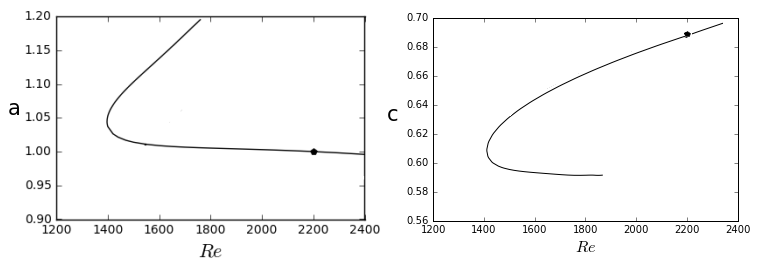
\includegraphics[width=0.9\linewidth]{autoref_contin.png}}
\caption{Продолжение модельного порыва по числу Рейнольдса}
\label{contin_pic}
\end{figure} 

В \textbf{разделе 4.2} приведены результаты продолжения модельного порыва по числу Рейнольдса. Продолжение модельного порыва по $\Re$ позволило получить новые условно периодические решения уравнений Навье-Стокса с пространственно локализованной структурой. Решение в процессе продолжения определяется значением $\Re$ однозначно. Значения амплитуды трехмерной составляющей движения $a$ и скорости перемещения вдоль трубы $c$ как функции $\Re$ приведены на рисунке \ref{contin_pic}. Точки на графиках соответствуют исходному решению. Решения принадлежат однопараметрическому множеству. При $\Re \approx 1400$ обнаружена точка бифуркации. При меньших $\Re$ решений не существует. При больших $\Re$ существует две ветви решений, то есть при каждом значении $\Re$ существует два решения, каждое из которых принадлежит свой ветви. Ветвь, которой принадлежит исходное решение, называют нижней. Вторую ветвь называют верхней. Для верхней ветви характера большая интенсивность пульсаций и меньшая скорость перемещения вдоль трубы. По этим и некоторым другим параметрам решения с верхней ветви приближаются к турбулентному порву. Результаты согласуются с (Avila et al. 2013). 

\begin{figure}
\center{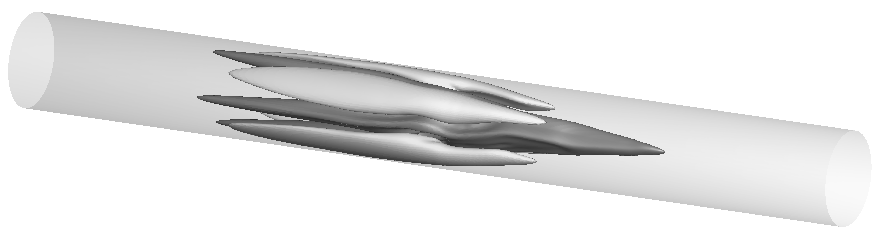
\includegraphics[width=0.9\linewidth]{autoref_3D_ub.png}}
\caption{Условно-периодическое решение с верхней ветви}
\label{3D_ub_pic}
\end{figure} 

В \textbf{разделе 4.3} выполнено исследование верхней ветви порожденного модельным порывом семейства условно-периодических решений. На рисунке \ref{3D_ub_pic} приведена визуализация мгновенного поля скорости решения с верхней ветви. Темным и светлым тоном представлены области пониженной и повышенной на $0.1U$ скорости относительно течения Пуазейля. Несмотря на существенные количественные отличия, решения с верхней ветви воспроизводят тот же механизм поддержания колебаний, что и решение с нижней ветви. Поле скорости решения представляется в виде суперпозиции средней и пульсационной составляющих. Области повышенной и пониженной средней скорости представляют собой вытянутые вдоль потока полосы. На рисунке \ref{ub_cs_pic}(a) приведены изолинии средней продольной скорости в поперечном сечении трубы. В центральной части расчетной области, где изолинии находятся на большем удалении от стенки, проходит полоса пониженной скорости. При больших и меньших значениях $\theta$ находятся полосы повышенной скорости. Пульсации возникают в результате линейной неустойчивости среднего течения между соседними полосами повышенной и пониженной скорости. Угловую неоднородность среднего течения поддерживают продольные вихри, которым соответствуют области повышенных и пониженных значений средней продольной завихренности $\Omega_x$. Распределение $\Omega^2_x$ по сечению трубы, в котором пульсации имеют существенную амплитуду, приведено на рисунке \ref{ub_cs_pic}(б). Определяющий вклад в производство $\Omega_x$ в уравнении \eqref{OX_eq} дают слагаемые \eqref{OXgen_terms}, описывающие нелинейное взаимодействие пульсаций продольной скорости и пульсаций продольной завихренности. Вклад слагаемых, соответствующих \eqref{OXgen_terms}, в производство $\Omega^2_x$ приведен на рисунке \ref{ub_cs_pic}(в). Механизм образования пульсаций продольной завихренности в области формирования продольных вихрей также аналогичен выделенному в модельном порыве. 


\begin{figure}
\center{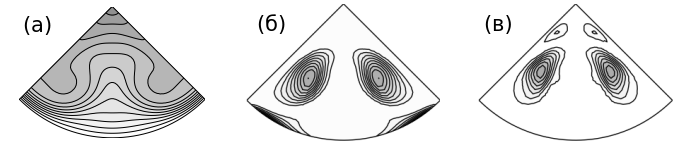
\includegraphics[width=0.9\linewidth]{ub_cs.png}}
\caption{Поле скорости решения с верхней ветви}
\label{ub_cs_pic}
\end{figure} 


\textbf{Раздел 4.4} посвящен анализу семейства трехмерных бегущей волн в течении Гагена-Пуазейля. Предельное решение на сепаратрисе, найденное, в отличии от модельного порыва, в непротяженной расчетной области, имеет вид бегущей волны. Продолжая это решение по числу Рейнольдса удалось получить семейство решений в виде бегущих волн. В отличии от модельного порыва, среднее поле скорости бегущей волны не зависит от продольной координаты, и полосы и продольные вихри имеют бесконечную протяженность. Несмотря на это, механизм поддержания колебаний в этом семействе решений аналогичен механизму поддержания колебаний в модельном порыве. Исключение составляет тот факт, что среднее поле скорости оказывается линейно устойчивым. Тем не менее, главная собственная функция линейной задачи устойчивости повторяет форму и фазовой скорость пульсационной составляющей движения, что дает основание полагать, что механизм поддержания колебаний и в этом случае является линейным. 

\textbf{Раздел 4.5} посвящен анализу двух семейств трехмерных бегущих волн в плоском течении Пуазейля. Постановка задачи в этом случае аналогична постановке задачи о течении в круглой трубе. Первое семейство решений порождено предельным решением на сепаратрисе, которое при некоторых параметрах имеет вид бегущей волны. Второе семейство порождено устойчивым при наложенных дополнительных условиях симметрии решением. Несмотря на существенные отличия, оба семейства воспроизводят общий с модельным порывом механизм поддержания колебаний. В некоторых случаях среднее поле скорости линейно устойчиво, но и в этих случаях главная собственная функция линейной задачи устойчивости повторяет форму и фазовую скорость пульсаций. В некоторых случаях слагаемое \eqref{ox1gen_main_terms} в уравнении \eqref{ox2_eq} оказывается не единственным, оказывающим существенное влияние на форму $\omega'_x$ в области расположения продольных вихрей. Тем не менее, именно это слагаемое порождает пульсации $\omega'_x$, согласованные с $v'_x$ необходимым для поддержания продольны вихрей образом, и именно это слагаемое имеет постоянное значение во всей области существования продольны вихрей. 

В \textbf{разделе 4.6} приведены выводы по главе. Основные результаты, приведенные в главе, опубликованы в работах автора диссертации \cite{Vest18, KMU2016}. 
